\documentclass{article}
\usepackage{graphicx}

\usepackage{amsmath}

\begin{document}

\begin{center}
	Quadrotor
\end{center}

%\begin{figure}[h]
%	\centering
%	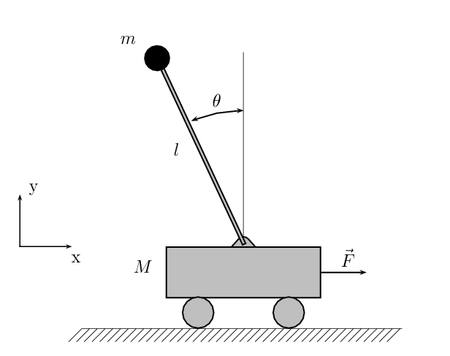
\includegraphics[scale=2]{Cart-pendulum.png}
%\end{figure}

Dynamics equation:

\begin{eqnarray}
	& \ddot{x} = -\frac{f_t}{m}[\sin \phi \sin \psi + \cos \phi \cos \psi \sin \theta] \\
	& \ddot{y} = -\frac{f_t}{m}[\cos \phi \sin \psi \sin \theta + \cos \psi \sin \phi] \\
	& \ddot{z} = g - \frac{f_t}{m}[\cos \phi \cos \theta]\\
	& \ddot{\phi} = \frac{I_y-I_z}{I_x}\dot{\theta}\dot{\psi} + \frac{\tau_x}{I_x}\\
	& \ddot{\theta} = \frac{I_z-I_x}{I_y}\dot{phi}\dot{\psi} + \frac{\tau_y}{I_y}\\
	& \ddot{\psi} = \frac{I_x-I_y}{I_z}\dot{\phi}\dot{\theta} + \frac{\tau_z}{I_z}
\end{eqnarray}
where 

$x$, $y$, $z$ are linear coordinates in reference frame ($z$ is a vertical coordinate)

$\phi$, $\theta$, $\psi$ are rp;;, pitch and yaw angles

$f_t$ is a thrust

$\tau_x$, $\tau_y$ and $\tau_z$ are force momentums

$m$ is a quadrotor mass

$g$ is a free fall  acceleration

$I_x$, $I_y$, $I_z$ are inertia momentums along respective axis of quadrotor

$l$ is the distance between any rotor and the center of the quadrotor

$b$ is the thrust coefficient

$d$ is the drag factor


Dependence between forces and velocities:

\begin{eqnarray}
	& f_t = b(\Omega_1^2 + \Omega_2^2 + \Omega_3^2 + \Omega_4^2) \\
	& \tau_x = bl(\Omega_3^2 - \Omega_1^2) \\
	& \tau_y = bl(\Omega_4^2 - \Omega_2^2) \\
	& \tau_z = d(\Omega_1^2 + \Omega_4^2 - \Omega_1^2 - \Omega_3^2)
\end{eqnarray}

where $\Omega$ is a velocity

\begin{eqnarray}
	& \Omega_1 = \sqrt{\frac{f_t - \frac{b}{d}\tau_z-\frac{2}{l}\tau_x}{4b}} \\
	& \Omega_2 = \sqrt{\frac{f_t + \frac{b}{d}\tau_z-\frac{2}{l}\tau_y}{4b}}  \\
	& \Omega_3 = \sqrt{\frac{f_t - \frac{b}{d}\tau_z +\frac{2}{l}\tau_x}{4b}}  \\
	& \Omega_4 = \sqrt{\frac{f_t + \frac{b}{d}\tau_z +\frac{2}{l}\tau_y}{4b}} 
\end{eqnarray}

	
\end{document}